\section{Problema 3: El se\~nor de los caballos}
\subsection{Descripci\'on de la problem\'atica}

En este problema, se presenta un tablero de ajedrez de tama\~no $nxn$, el cual cuenta con alguna cantidad de caballos ubicados en una posici\'on aleatoria del tablero. Lo que se quiere lograr es \emph{cubrir} todo el tablero. Un casillero se considera cubierto si hay un caballo en \'el o bien, si es una posici\'on en la cual alg\'un caballo existente puede moverse con un s\'olo movimiento. Para lograr este cometido, puede ser necesario agregar nuevas fichas \emph{caballo} al tablero. No existe un l\'imite en la cantidad de caballos para agregar, pero lo que se busca es dar una soluci\'on con la m\'inima cantidad de caballos posibles.\\


En la figura \ref{caballito} se pueden ver todas las casillas que est\'an cubiertas por un s\'olo caballo.


 \begin{figure}[h!]
   \begin{center}
 	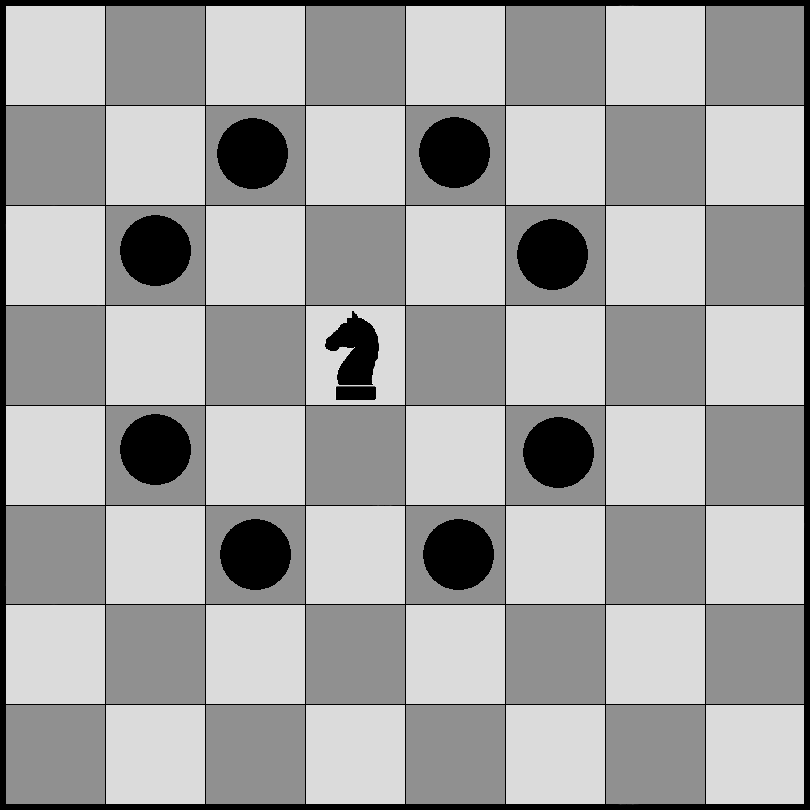
\includegraphics[scale=0.3]{imagenes/ej3/caballito.png}
 	\caption{Casillas que \emph{cubre} un caballo}
 	\label{caballito}	
   \end{center}
 \end{figure}



\newpage
\subsection{Resoluci\'on propuesta y justificaci\'on}

%re jodido esto amigooooo
%se ahcen todas las combinaciones y se va guardando la que tenga menor cantidad de caballos?
\newpage
\subsection{An\'alisis de la complejidad}
\newpage
\subsection{C\'odigo fuente}
\newpage
\subsection{Experimentaci\'on}


\subsubsection{Constrastaci\'on Emp\'irica de la complejidad}
-Hacer lo que hicieron en clase\\
\newpage
